\documentclass[11pt,a4paper]{article}

\usepackage[margin=1in]{geometry}
\usepackage{titlesec}
\usepackage{enumitem}
\usepackage{hyperref}
\usepackage{parskip}
\usepackage{graphicx}
\usepackage{float}
\usepackage{booktabs}
\usepackage{amsmath}

\hypersetup{colorlinks=true, linkcolor=blue, urlcolor=blue}

\titleformat{\section}{\large\bfseries}{\thesection}{0.5em}{}
\titleformat{\subsection}{\normalsize\bfseries}{\thesubsection}{0.5em}{}
\setlist{leftmargin=1.4em, topsep=2pt, itemsep=2pt}

\title{\vspace{-1.5cm}\textbf{PKCERT AI \& Software Development Internship \\ Task 09: Support Vector Machines \& k-Nearest Neighbors}}
\author{Abdullah Amir}
\date{AI and Software Development \\ 14 July 2026}

\begin{document}

\maketitle
\vspace{-0.8cm}

This report covers the theory and the results for two classifiers, a Support
Vector Machine and a k-Nearest Neighbors model. The full code, outputs and plots
live in the notebook \texttt{svm\_knn.ipynb}. The dataset is the \textbf{UCI Raisin}
set: 900 raisins of two Turkish varieties, \textbf{Kecimen} and \textbf{Besni},
described by 7 numeric shape features pulled from images (area, perimeter, the two
axis lengths, eccentricity, convex area and extent). The goal is to tell the two
varieties apart from shape alone. I picked this one on purpose because it is a bit
off the beaten track, it is perfectly balanced at 450 raisins per class, and the
features sit on wildly different scales: area runs into the tens of thousands while
extent hovers around 0.7. That scale gap is exactly what makes it a good test for
these two algorithms, since both of them measure distances and both fall apart if
you skip feature scaling.

% ----------------------------------------------------------------
\section*{Part A: Dataset Selection \& Preparation}

The raisin data comes clean, with no missing values and no categorical columns to
encode, so the only real preparation is the target and the scaling. I encode the
label as Besni = 1 (the positive class) and Kecimen = 0. Then I split the data
80/20 with stratification, so both the training and test sets keep the even 50/50
split, which leaves 720 raisins for training and 180 for testing.

\textbf{Scaling is the step that matters here.} Both SVM and kNN work off distances
between points, and when one feature (area, in the tens of thousands) dwarfs
another (extent, near 0.7), that big feature drowns out everything else and the
model effectively ignores the rest. I fit a \texttt{StandardScaler} on the training
set only, so each feature ends up with mean 0 and standard deviation 1, and then
apply that same scaler to the test set. Fitting on the training data alone keeps
the test set genuinely unseen and avoids leaking information.

\begin{figure}[H]
    \centering
    
\includegraphics[width=0.92\textwidth]{figures/01_dataset_overview.png}
    \caption{Left: the perfectly balanced classes. Right: the raw feature scales on
    a log axis, showing why scaling is not optional here. Area and convex area are
    four orders of magnitude larger than extent and eccentricity.}
\end{figure}

% ----------------------------------------------------------------
\section*{Part B: Support Vector Machine}

\textbf{Working principle.} An SVM looks for the boundary that separates the two
classes with the widest possible \textbf{margin}, the empty gap on either side of
the line. Only the points sitting right on the edge of that gap, the
\textbf{support vectors}, actually decide where the boundary goes, which is why the
model is named after them. The margin is found by solving
\[ \min_{w,b}\ \tfrac{1}{2}\lVert w\rVert^2 \quad\text{subject to}\quad y_i(w^\top x_i + b) \ge 1, \]
and a soft-margin version relaxes those constraints with a penalty $C$ so a few
points are allowed to sit inside the margin or on the wrong side. A small $C$ gives
a wider, more forgiving margin, and a large $C$ tries harder to classify every
training point correctly, at the risk of overfitting.

\textbf{Choice of kernel.} When the classes are not separable by a straight line,
the \textbf{kernel trick} maps the data into a higher dimensional space where a
linear boundary does exist, without ever computing those coordinates explicitly.
I use the \textbf{RBF (Gaussian) kernel} as the default, because it is the usual
first choice when you do not know the shape of the boundary in advance and it can
bend around non-linear patterns. Out of interest I also tried a linear kernel: it
scored 0.928 on this split, marginally ahead of the RBF's 0.911, which tells us the
two raisin varieties are very nearly linearly separable in the scaled feature
space. I kept the RBF as the headline model since it is the more general choice and
the difference is within the noise of a single split.

\textbf{Results.} The RBF SVM scored accuracy \textbf{0.911}, precision 0.963,
recall 0.856 and F1 0.906 on the test set. The four metrics come from the confusion
matrix, whose cells are true negatives (TN), false positives (FP), false negatives
(FN) and true positives (TP):
\begin{itemize}
    \item \textbf{Accuracy} $=(TP+TN)/\text{all}$, the overall share of correct
    calls. It is a fair headline here because the classes are balanced.
    \item \textbf{Precision} $=TP/(TP+FP)$. Of the raisins we labelled Besni, how
    many really were. At 0.963 the model almost never cries Besni wrongly.
    \item \textbf{Recall} $=TP/(TP+FN)$. Of the true Besni raisins, how many we
    caught. At 0.856 it misses a few more, which is the model's weaker side.
    \item \textbf{F1} $=2PR/(P+R)$, the harmonic mean, which only stays high when
    precision and recall are both high.
\end{itemize}
The confusion matrix shows the split of mistakes: just 3 Kecimen wrongly called
Besni, against 13 Besni missed and called Kecimen. So when this SVM says Besni you
can trust it, but it plays it safe and lets a handful of real Besni slip through.

\begin{figure}[H]
    \centering
    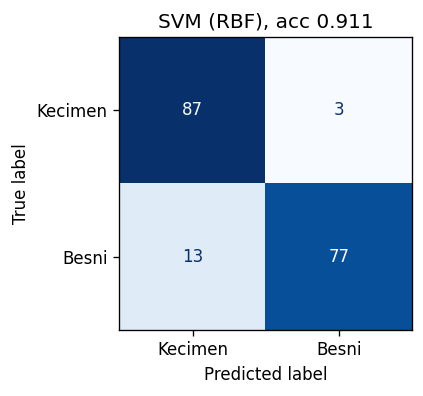
\includegraphics[width=0.46\textwidth]{figures/02_confusion_svm.png}
    \caption{SVM (RBF) confusion matrix. Rows are the true variety, columns the
    prediction. The 13 in the bottom-left (Besni called Kecimen) is where the
    recall is lost.}
\end{figure}

\textbf{Advantages, limitations and applications.} SVMs are strong in high
dimensions, they cope well when there are more features than samples, and because
only the support vectors matter they are memory efficient once trained. The catch
is that they do not scale nicely to very large datasets, the result depends heavily
on getting $C$ and the kernel right, and a plain SVM gives you a hard label rather
than a probability. You see them in text and image classification, handwriting
recognition, bioinformatics such as protein and cancer classification, and, close
to home for PKCERT, in spam filtering and network intrusion detection.

% ----------------------------------------------------------------
\section*{Part C: k-Nearest Neighbors}

\textbf{Working principle.} kNN is about as simple as a classifier gets, and it
does no real training at all. To label a new raisin it measures the distance
(Euclidean here) to every raisin in the training set, picks the \textbf{K} closest
ones, and takes a majority vote of their varieties. That is the whole algorithm.
All the work happens at prediction time, which is why it is called a lazy learner.
Because every step is a distance, feature scaling is just as essential as it was for
the SVM.

\textbf{Choosing K.} K is the one knob that matters. Too small (K = 1) and the model
clings to every noisy point and overfits; too large and it smooths across the
boundary and starts ignoring genuine local structure. Rather than guess, I swept K
from 1 to 25 and scored each value with 5-fold cross-validation on the training set.
The best result came at \textbf{K = 8}, so that is what I used. Even values are fine
here because the two classes rarely tie in an 8-way vote.

\begin{figure}[H]
    \centering
    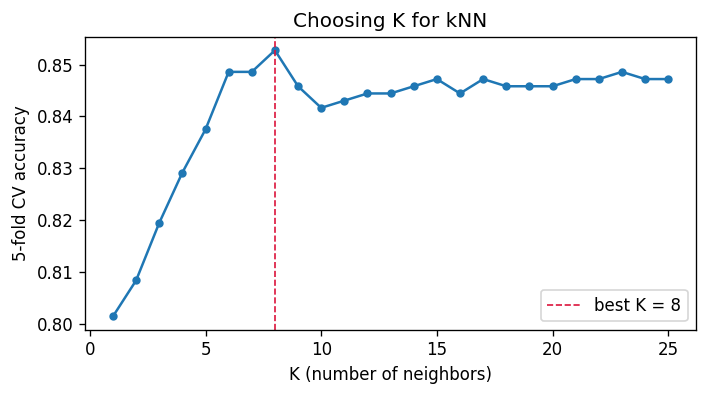
\includegraphics[width=0.6\textwidth]{figures/03_knn_k_sweep.png}
    \caption{Cross-validation accuracy against K. It climbs quickly out of the noisy
    low-K region and settles into a broad plateau, peaking at K = 8.}
\end{figure}

\textbf{Results.} With K = 8 the kNN scored accuracy \textbf{0.861}, precision 0.945,
recall 0.767 and F1 0.847. The same pattern as the SVM shows up, only stronger: very
high precision but noticeably lower recall. Its confusion matrix has 4 Kecimen
called Besni against 21 Besni missed, so it is even more cautious about the Besni
class than the SVM was, and pays for it with 8 extra mistakes overall.

\begin{figure}[H]
    \centering
    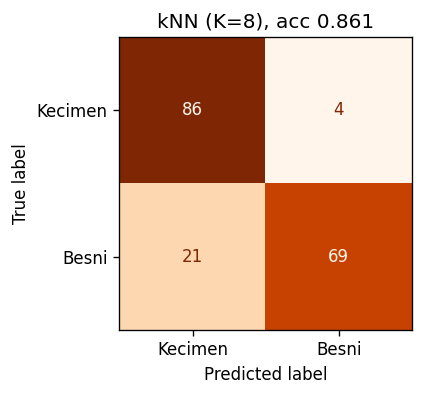
\includegraphics[width=0.46\textwidth]{figures/04_confusion_knn.png}
    \caption{kNN (K = 8) confusion matrix. The 21 missed Besni in the bottom-left
    is the main gap between this model and the SVM.}
\end{figure}

\textbf{Advantages, limitations and applications.} kNN is trivial to understand, has
nothing to train, and naturally handles multi-class problems and non-linear
boundaries. Its weaknesses are the flip side of that simplicity: prediction is slow
and memory hungry because it has to keep and search the whole training set every
time, it suffers badly in high dimensions (the curse of dimensionality), and it is
very sensitive to scaling and to irrelevant features. It shows up in recommender
systems, pattern and image recognition, and anomaly detection.

% ----------------------------------------------------------------
\section*{Part D: Comparative Analysis}

Putting the two side by side on the same test set, and then backing it up with
5-fold cross-validation on the whole pipeline, gives a steadier read than any single
number.

\begin{table}[H]
\centering
\begin{tabular}{lrrrrr}
\toprule
\textbf{Model} & \textbf{Accuracy} & \textbf{Precision} & \textbf{Recall} & \textbf{F1} & \textbf{CV acc (std)} \\
\midrule
SVM (RBF kernel) & 0.911 & 0.963 & 0.856 & 0.906 & 0.868 (0.021) \\
kNN (K = 8)      & 0.861 & 0.945 & 0.767 & 0.847 & 0.847 (0.014) \\
\bottomrule
\end{tabular}
\caption{Test-set metrics plus 5-fold cross-validation accuracy on the full scaled
dataset. The SVM leads on every metric except cross-validation stability.}
\end{table}

\begin{figure}[H]
    \centering
    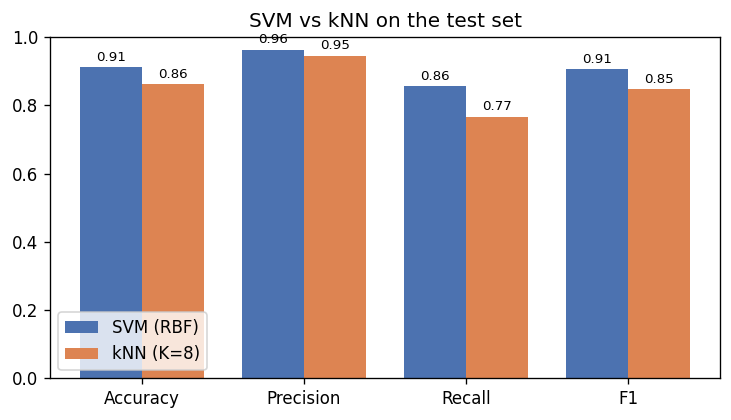
\includegraphics[width=0.7\textwidth]{figures/05_model_comparison.png}
    \caption{The four headline metrics side by side. The two models are close on
    precision but the SVM pulls clearly ahead on recall, and therefore on F1 and
    accuracy.}
\end{figure}

\textbf{Reading the results.} The SVM wins on every headline metric: it is 5 points
more accurate, and the whole gap comes from recall, where it catches 77 of the 90
Besni raisins against the kNN's 69. Both models are cautious about the Besni class,
but the SVM is less so. Cross-validation confirms the ranking rather than
overturning it, unlike Day 08 where the single split had been misleading: the SVM
averages 0.868 accuracy across five folds against the kNN's 0.847. The kNN's folds
are very slightly tighter (std 0.014 versus 0.021), so it is a touch more consistent,
but not by enough to make up a 2 point deficit in the mean.

\textbf{Recommendation.} \emph{For this dataset I recommend the SVM with an RBF
kernel.} It is more accurate on the held-out test set, it holds that lead under
cross-validation, and it recovers noticeably more of the Besni raisins that both
models tend to miss. It is also the better fit for the data on principle: with only
7 clean numeric features and 900 rows this is a small, low-dimensional problem where
an SVM is right at home and where kNN's slow, memory-hungry prediction buys you
nothing. kNN remains a perfectly reasonable, dead-simple baseline, and the fact that
it lands within a few points of the SVM tells us the two varieties really are fairly
easy to separate once the features are scaled. If a fully transparent, explain-it-in-
one-sentence model mattered more than the last few points of accuracy, kNN would be
the pick.

\vspace{0.4cm}
The notebook and README are on GitHub:
\url{https://github.com/AbdullahAmir06/ai-internship-abdullahamir}.

\end{document}
